\addcontentsline{toc}{subsubsection}{Illustrations: Applications of Derivatives}
\vbtitle{\textbf{Illustrations: Applications of Derivatives}}
\BgThispage
\begin{enumerate}
    \item For the given graph, find out the slope of the tangent at $x=\pi$ and also the equation of tangent?
        \begin{center}
            \begin{tikzpicture}
            \tzaxes(-0.5, -0.5)(6, 2){$x$}{$y$}
            \tzfn{sin(deg(\x))}[0:1.5*pi]{$f(x) = \sin x$}[r]
            \end{tikzpicture}
        \end{center}
        \begin{solution}
            \begin{align*}
                f(x) &= \sin x\\
                \frac{df}{dx} &= \cos x\\
                \frac{df}{dx}\bigg|_{x=\pi} &= \cos \pi = -1\\
                \intertext{The slope of the tangent at $x=\pi$ is $-1$.}
                \intertext{The equation of the tangent is given by:}
                y - y_1 &= m(x-x_1)\\
                y - \sin \pi &= -1(x-\pi)\\
                y - 0 &= -x + \pi\\
                \Aboxed{y &= -x + \pi}
            \end{align*}
        \end{solution}

    \item For the given graph, what would the slope of the tangent at $x=1$ ?
        \begin{center}
            \begin{tikzpicture}
            \tzaxes(-1, -1)(4, 3){$x$}{$y$}
            \tzfn{\x*\x -2*\x}[-1:3]{$f(x) = x^2-2x$}[r]
            \end{tikzpicture}
        \end{center}
        \begin{solution}
            \begin{align*}
                f(x) &= x^2 - 2x\\
                \frac{df}{dx} &= 2x - 2\\
                \frac{df}{dx}\bigg|_{x=1} &= 2(1) - 2 = 0\\
                \intertext{The slope of the tangent at $x=1$ is $0$.}
            \end{align*}
        \end{solution}

    \item For the given $v-t$ graph, Find the acceleration at $t=2s$. \\
    Acceleration is defined as the rate of change of velocity with respect to time.
        \begin{center}
            \begin{tikzpicture}
                \tzaxes[->](-1, -1)(5, 3){$t$}{$v$}
                \tztos"curve"(0, 0)[out=0, in=180]
                            (2, 2)[out=0, in=180]
                            (4, 1);
                \tzvXpointat{curve}{2}(A)
                \tzslopeat[->, red]{curve}{2}{1.5cm}
                \tzprojx*[dashed](A){$2$}
            \end{tikzpicture}
        \end{center}
        \begin{solution}
            \begin{align*}
                \intertext{We can represent rate change with the held of derivative.}
                a &= \dfrac{dv}{dt}\\
                \intertext{From the given graph, we can see that slope of the tangent at $t=2$ is $0$.}
                \intertext{So, the acceleration at $t=2$ is $0$.}
            \end{align*}
        \end{solution}
    
\BgThispage
    \item For the given $v-s$ graph, find the acceleration at $s=2\m$. \\
        \begin{center}
            \begin{tikzpicture}
                \tzaxes[->](-1, -1)(5, 3){$s$}{$v$}
                \tztos"curve"(0, 0)[out=0, in=250]
                            (3, 2.5);
                \node at (3, 2.5)[right]{$v=\dfrac{s^2}{2}$};
                \tzvXpointat{curve}{2}(A)
                \tzslopeat[->, red]{curve}{2}{2cm}
                \tzprojx*[dashed](A){$2$}
            \end{tikzpicture}
        \end{center}
        \begin{solution}
            \begin{align*}
                \intertext{We can represent rate change with the held of derivative.}
                a &= \dfrac{dv}{dt}\\
                \intertext{But here, we have $v$ as a function of $s$. So, we can write it as:}
                a &= \dfrac{dv}{ds} \times \dfrac{ds}{dt}\\
                a &= v \times \dfrac{dv}{ds}
                \intertext{$v$ at $s=2$ is:}
                v &= \dfrac{s^2}{2}=\dfrac{2^2}{2} = 2
                \intertext{Now, we can find the derivative of $v$ with respect to $s$.}
                \dfrac{dv}{ds}\bigg|_{s=2} &= \dfrac{d}{ds}\left(\dfrac{s^2}{2}\right)= \dfrac{1}{2} \times 2s = 2\\
                \intertext{Now, we can find the acceleration at $s=2$.}
                a &= 2 \times 2 = 4
            \end{align*}
        \end{solution}

        \vbstarednote{In the above examples, we haven't paid attention to the units. But you can consider every quantity in SI units.}
\end{enumerate}